\section{Casi d'Uso}\label{CasiUso}
\subsection{Introduzione}\label{CasiUso_Introduzione}
Nella seguente sezione verranno identificati i casi d'uso che abbiamo individuato.\\
Il numero di casi cha abbiamo analizzato è limitato poiché il plug-in fornisce funzionalità aggiuntive ad una piattaforma preesistente, per la quale non è fornita documentazione in quanto già disponibile presso il sito web del fornitore della piattaforma: \textit{Grafana Labs}.

\subsection{Attori}\label{Attori}
E' importante notare che il numero esiguo di differenti attori che possono approcciarsi al prodotto in esame è principalmente dovuto al fatto che, essendo il progetto "G\&B" un plug-in di un sistema indipendente, poche tipologie di utenti possono effettivamente approcciarsi al prodotto finale.\\
E' altrettanto importante sottolineare che il sistema di registrazione ed autenticazione dell'utente viene gestito interamente dal sistema \textit{Grafana}, dal momento che, ovviamente, il prodotto finale non avrà una funzionalità di autenticazione interna.

\subsubsection*{Attori Primari}
\begin{itemize}
\item \textbf{Utente:} si riferisce ad un generico utente che ha effettuato l'autenticazione al sistema \textit{Grafana}. E' l'unica tipologia di utente con facoltà di interagire con il prodotto, in quanto questo risulta essere un plug-in.
\end{itemize}

\subsubsection*{Attori Secondari}
\begin{itemize}
\item \textbf{Piattaforma \textit{Grafana}:} sistema di monitoraggio di flusso dati, di cui il prodotto da realizzare è un plug-in. Consente agli utenti autenticati, attraverso funzionalità proprie, di realizzare grafici ed alert riferiti a dati forniti dal plug-in.
\end{itemize}

%\begin{itemize}
%\item \textbf{Attore Primario:}
%\item \textbf{Precondizioni:}
%	\begin{enumerate}
% \item
% \end{enumerate}
%\item \textbf{Postcondizioni:}
% \begin{enumerate}
% \item
% \end{enumerate}
%\item \textbf{Scenario Principale:}
% \begin{enumerate}
% \item
% \end{enumerate}
%\item \textbf{Estensioni:}
%\end{itemize}

\subsection{UC1 - Aggiunta della Rete Bayesiana al Plug-in G\&B}\label{UC1}

\begin{figure}[H]
	\begin{center}
		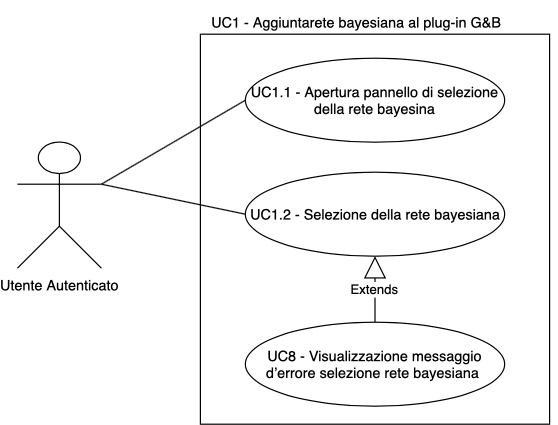
\includegraphics[scale=0.5]{./images/UC1.png}
		 \caption{UC1 - Aggiunta della Rete Bayesiana al Plug-in G\&B}	
	\end{center}
\end{figure}
\begin{itemize}
	\item \textbf{Attore Primario}: Utente;
	\item \textbf{Precondizioni}: l'utente deve aver effettuato il login nella piattaforma \textit{Grafana}, deve aver selezionato una dashboard e aggiunto il pannello "G\&B";
	\item \textbf{Postcondizioni}: l'utente ha aggiunto la rete bayesiana al plug-in. Attraverso \hyperref[UC2]{UC2 (§\ref*{UC2})} può selezionare quali nodi sorgente collegare alla rete.
	\item \textbf{Scenario Principale:}
	\begin{enumerate}
		\item L'utente seleziona e clicca sul bottone denominato "Carica Rete Bayesiana" (\hyperref[UC1.1]{UC1.1 (§\ref*{UC1.1})});
		\item L'utente si trova davanti una finestra presso cui selezionare il file \textit{.JSON} contenente la definizione della rete (\hyperref[UC1.2]{UC1.2 (§\ref*{UC1.2})}) e seleziona "Aggiungi".
	\end{enumerate}
	\item \textbf{Estensioni:} \hyperref[UC8]{UC8 (§\ref*{UC8})} estende \hyperref[UC1.2]{UC1.2 (§\ref*{UC1.2})}: l'utente visualizza un messaggio di errore nel caso in cui l'operazione non sia andata a buon fine.
\end{itemize}

\subsubsection{UC1.1 - Apertura Pannello di Selezione della Rete Bayesiana}\label{UC1.1}
\begin{itemize}
	\item \textbf{Attore Primario}: Utente; 
	\item \textbf{Precondizioni}: l'utente visualizza il pannello "G\&B" nella dashboard.
	\item \textbf{Postcondizioni}: l'utente ha cliccato il bottone con etichetta "Aggiungi Rete Bayesiana" e visualizza il pannello per la selezione del file della rete;
	\item \textbf{Scenario Principale}: l'utente clicca il pulsante con etichetta "Aggiungi Rete Bayesiana" nel pannello "G\&B Panel" nella dashboard.
\end{itemize}


\subsubsection{UC1.2 - Selezione della Rete Bayesiana}\label{UC1.2}
\begin{itemize}
	\item \textbf{Attore Primario}: Utente;
	\item \textbf{Precondizioni}: l'utente ha cliccato il bottone con etichetta "Aggiungi Rete Bayesiana";
	\item \textbf{Postcondizioni}: l'utente ha selezionato la rete bayesiana desiderata e ha premuto il pulsante con etichetta "Aggiungi";
	\item \textbf{Scenario Principale}:
	\begin{enumerate}
		\item L'utente seleziona dalla finestra il file da importare;
		\item L'utente clicca il pulsante con etichetta "Aggiungi".
	\end{enumerate}
	\item \textbf{Estensioni:} \hyperref[UC8]{UC8 (§\ref*{UC8})}: l'utente visualizza un messaggio di errore nel caso in cui l'operazione di caricamento del file non sia andata a buon fine.
\end{itemize}

\pagebreak

\subsection{UC2 - Collegamento Nodi al Flusso Dati}\label{UC2}

\begin{figure}[H]
\centering
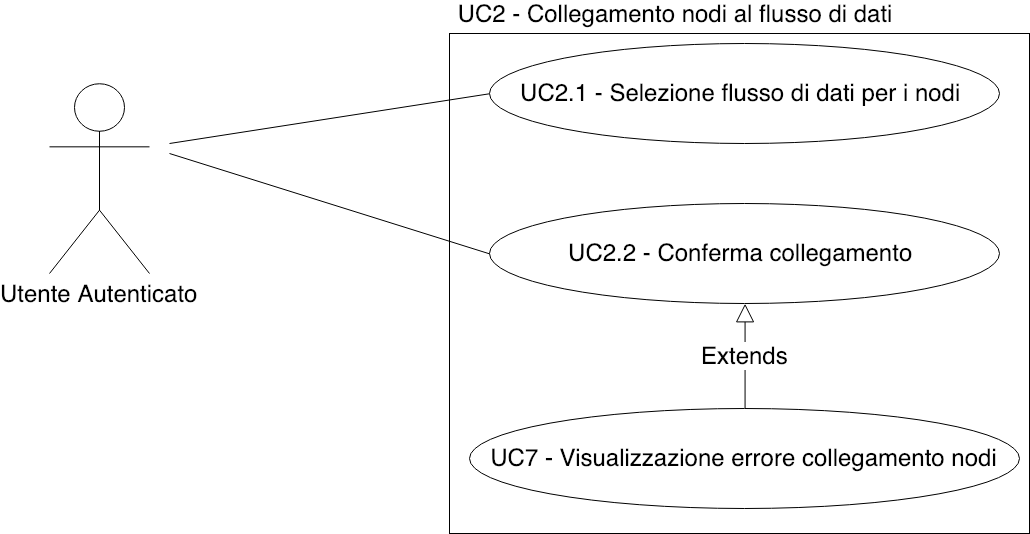
\includegraphics[scale=0.5]{./images/UC2.png}
\caption{UC2 - Collegamento Nodi della Rete Bayesiana al Flusso Dati}
\end{figure}

\begin{itemize}
\item \textbf{Attore Primario}: Utente;
\item \textbf{Precondizione}: l'utente ha caricato con successo la rete bayesiana (\hyperref[UC1]{UC1 (§\ref*{UC1})});
\item \textbf{Postcondizioni}: 
	\begin{enumerate}
	\item L'utente ha collegato con successo i nodi desiderati della rete bayesiana caricata in \hyperref[UC1]{UC1 				(§\ref*{UC1})};
	\item Il pannello usato per il collegamento dei nodi non è più interagibile, tranne il pulsante "Modifica 							Collegamento Nodi".
	\end{enumerate}
\item \textbf{Scenario Principale}:
	\begin{enumerate}
	\item (\hyperref[UC2.1]{UC2.1 (§\ref*{UC2.1})}) l'utente visualizza la lista di nodi che costituiscono la rete bayesiana caricata in \hyperref[UC1]{UC1(§\ref*{UC1})};
	\item (\hyperref[UC2.2]{UC2.2 (§\ref*{UC2.2})}) l'utente collega i nodi desiderati ad un flusso dati;
	\item (\hyperref[UC2.3]{UC2.3 (§\ref*{UC2.3})}) l'utente conferma il collegamento dei nodi.
	\end{enumerate}
\item \textbf{Estensioni}: \hyperref[UC9]{UC9 (§\ref*{UC9})} estende \hyperref[UC2.3]{UC2.3 (§\ref*{UC2.3})}: l'utente visualizza un messaggio di errore nel caso in cui non abbia collegato alcun nodo al flusso dati.
\end{itemize}

\subsubsection{UC2.1 - Visualizzazione della Lista dei Nodi della Rete Bayesiana e Rispettivi Stati}\label{UC2.1}
\begin{itemize}
\item \textbf{Attore Primario:}  Utente
\item \textbf{Precondizione:} l'utente ha caricato con successo la rete bayesiana (\hyperref[UC1]{UC1 									(§\ref*{UC1})});
\item \textbf{Postcondizione:} l'utente visualizza la lista di nodi di cui la rete bayesiana è costituita, vengono 			inoltre visualizzati gli stati di ogni nodo (collegato ad un flusso dati oppure no);
\item \textbf{Scenario Principale:}
	\begin{enumerate}
	\item L'utente visualizza una lista contenente i nominativi associati ad ogni nodo della rete bayesiana caricata 				in \hyperref[UC1]{UC1(§\ref*{UC1})};
	\item L'utente visualizza, accanto ai nominativi dei nodi, una lista di checkbox\glossario associate. Tali checkbox 							rappresentano lo stato del nodo a cui sono associate: "V" nel caso il nodo sia collegato ad un flusso dati, "X" 		altrimenti.
	\end{enumerate}
\end{itemize}

\pagebreak

\subsubsection{UC2.2 - Selezione Flusso di Dati e Livello di Soglia per il Nodo}\label{UC2.2}

\begin{figure}[H]
\centering
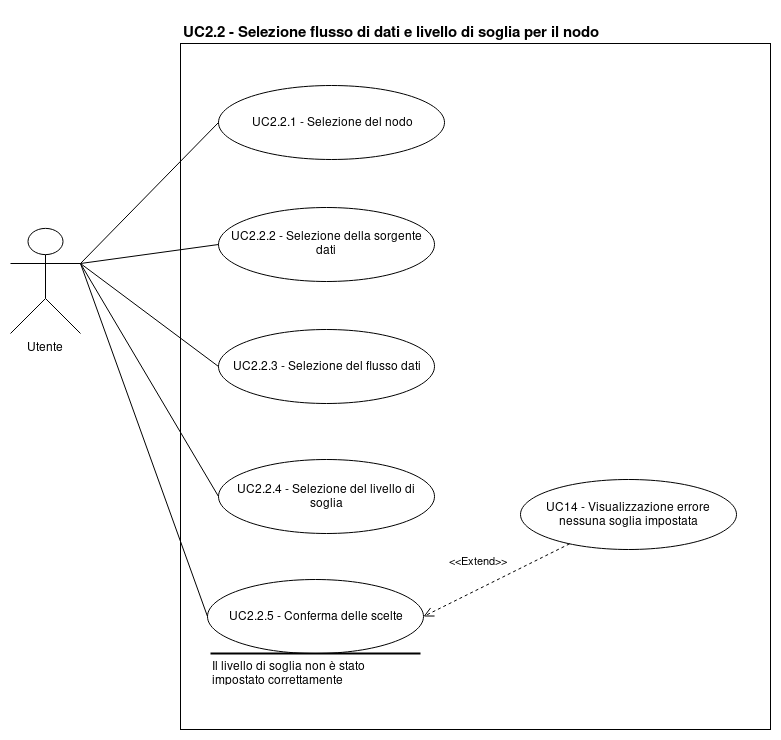
\includegraphics[scale=0.5]{./images/UC2-2.png}
\caption{UC2.2 - Selezione Flusso di Dati e Livello di Soglia per il Nodo}
\end{figure}

\begin{itemize}
\item \textbf{Attore Primario}: Utente;
\item \textbf{Precondizioni}: 
\begin{enumerate}
	\item L'utente ha caricato con successo la rete bayesiana (\hyperref[UC1]{UC1(§\ref*{UC1})});
	\item L'utente ha visualizzato la lista di nodi di cui la rete bayesiana è costituita ed il corrispondente stato 			(\hyperref[UC2.1]{UC2.1 (§\ref*{UC2.1})}).
\end{enumerate}
\item \textbf{Postcondizioni}: 
	\begin{enumerate}
	\item L'utente ha collegato il nodo desiderato ad uno e un solo flusso dati, impostandone correttamente per ogni possibile stato un livello di soglia al di sotto, o al di sopra, del quale la probabilità associata a quel dato stato risulta pari al 100\%, mentre le probabilità associate agli altri stati risultano pari allo 0\%;
	\item Se lo desidera, e vi sono ancora nodi a disposizione, l’utente può selezionare un altro nodo per il collegamento, o modificare le impostazioni di nodi già collegati.
	\end{enumerate}
\item \textbf{Scenario Principale}:
 \begin{enumerate}
 \item (\hyperref[UC2.2.1]{UC2.2.1 (§\ref*{UC2.2.1})}) Selezione del nodo;
 \item (\hyperref[UC2.2.2]{UC2.2.2 (§\ref*{UC2.2.2})}) Selezione della sorgente dati;
 \item (\hyperref[UC2.2.3]{UC2.2.3 (§\ref*{UC2.2.3})}) Selezione del flusso dati;
 \item (\hyperref[UC2.2.4]{UC2.2.4 (§\ref*{UC2.2.4})}) Selezione del livello di soglia;
 \item (\hyperref[UC2.2.5]{UC2.2.5 (§\ref*{UC2.2.5})}) Conferma delle scelte.
 \end{enumerate}
\item \textbf{Estensioni:} \hyperref[UC14]{UC14 (§\ref*{UC14})} estende \hyperref[UC2.2.5]{UC2.2.5 (§\ref*{UC2.2.5})}: l'utente visualizza un messaggio di errore nel caso in cui non abbia impostato correttamente 	un livello di soglia per il nodo selezionato.
\end{itemize}

\paragraph{UC2.2.1 - Selezione del Nodo}\label{UC2.2.1}
\begin{itemize}
\item \textbf{Attore Primario:} Utente;
\item \textbf{Precondizione:} l'utente ha visualizzato la lista di nodi di cui la rete bayesiana è costituita ed il 	corrispondente stato (\hyperref[UC2.1]{UC2.1 (§\ref*{UC2.1})});
\item \textbf{Postcondizione:} l'utente visualizza una finestra contenente un menù a tendina in cui è possibile selezionare la sorgente dei dati e una lista di tutti i possibili stati del nodo selezionato;
\item \textbf{Scenario Principale:} l'utente clicca il nominativo del nodo che desidera collegare ad un certo flusso dati.
\end{itemize}

\paragraph{UC2.2.2 - Selezione della Sorgente Dati}\label{UC2.2.2}
\begin{itemize}
\item \textbf{Attore Primario:} Utente;
\item \textbf{Precondizione:} l'utente ha selezionato il nodo che desidera collegare ad un certo flusso dati 					(\hyperref[UC2.2.1]{UC2.2.1 (§\ref*{UC2.2.1})});
\item \textbf{Postcondizioni:} 
	\begin{enumerate}
	\item L'utente ha selezionato la sorgente dati;
	\item L'utente visualizza una lista di flussi dati a cui è possibile 	collegare il nodo selezionato.
	\end{enumerate}
\item \textbf{Scenario Principale:} l'utente seleziona, attraverso un menù a tendina, la sorgente dati.
\end{itemize}

\paragraph{UC2.2.3 - Selezione del Flusso Dati}\label{UC2.2.3}
\begin{itemize}
\item \textbf{Attore Primario:} Utente;
\item \textbf{Precondizione:} l'utente ha selezionato la sorgente dei dati (\hyperref[UC2.2.2]{UC2.2.2 (§\ref*{UC2.2.2})});
\item \textbf{Postcondizioni:}
	\begin{enumerate}
	\item L'utente ha selezionato il flusso dati a cui collegare il nodo desiderato;
	\item L'utente visualizza un'estensione della finestra contenente i flussi dati disponibili, attraverso cui è 					possibile impostare un livello di soglia;
	\end{enumerate}
\item \textbf{Scenario Principale:} l'utente seleziona, attraverso un click, il flusso dati a cui desidera 						collegare il nodo in esame.
\end{itemize}

\paragraph{UC2.2.4 - Selezione del Livello di Soglia}\label{UC2.2.4}
\begin{itemize}
\item \textbf{Attore Primario:} Utente
\item \textbf{Precondizione:} l'utente ha selezionato il nodo che desidera collegare ad un certo flusso dati 					(\hyperref[UC2.2.1]{UC2.2.1 (§\ref*{UC2.2.1})});
\item \textbf{Postcondizione:} l'utente ha impostato, per ogni stato del nodo, un livello di soglia al di sotto, o al di sopra,	del quale la probabilità associata a quel dato stato risulta pari al 100\%, mentre le probabilità associate agli altri stati risultano pari allo 0\%;
\item \textbf{Scenario Principale:}
	\begin{enumerate}
	\item L'utente visualizza, associati al nominativo di ogni possibile stato del nodo, una sezione composta di tre campi dati che devono essere obbligatoriamente riempiti;
	\item Per ogni stato del nodo l'utente digita, nel primo campo editabile, il valore numerico del livello di soglia;
	\item Per ogni stato del nodo l'utente seleziona, attraverso una casella a scelta multipla, se il valore numerico impostato sia un valore di massimo oppure di minimo;
	\item Per ogni stato del nodo l'utente seleziona, attraverso una checkbox, se la soglia definita sia critica o meno. Nel caso in cui si tratti di una soglia critica, qualora dovessero essere monitorati valori che la facciano scattare, si attiverebbe immediatamente l'attività di ricalcolo delle probabilità in sede di monitoraggio e visualizzazione dati (\hyperref[UC4.2]{UC4.2 (§\ref*{UC4.2})}).
	\end{enumerate}
\end{itemize}

\paragraph{UC2.2.5 - Conferma delle Scelte}\label{UC2.2.5}
\begin{itemize}
\item \textbf{Attore Primario:} Utente;
\item \textbf{Precondizioni:}
	\begin{enumerate}
	\item L'utente ha selezionato un flusso dati a cui collegare il nodo in esame (\hyperref[UC2.2.3]{UC2.2.3 							(§\ref*{UC2.2.3})});
	\item L'utente ha impostato correttamente un livello di soglia al di sotto, o al di sopra, 	del quale la probabilità associata a quel dato stato risulta pari al 100\%, mentre le probabilità associate agli altri stati risultano pari allo 0\% (\hyperref[UC2.2.4]{UC2.2.4 (§\ref*{UC2.2.4})});
	\end{enumerate}
\item \textbf{Postcondizioni:}
	\begin{enumerate}
	\item La finestra comparsa, per consentire all'utente di compiere le operazioni necessarie al fine di collegare il 		nodo ad un flusso dati, scompare;
	\item La checkbox corrispondente al nodo appena collegato passa dallo stato "X", che rappresenta un nodo non 					collegato, allo stato "V";
	\end{enumerate}
\item \textbf{Scenario Principale:} l'utente clicca il pulsante "Conferma scelte";
\item \textbf{Estensioni:} \hyperref[UC14]{UC14 (§\ref*{UC14})}: nel caso in cui il valore numerico inserito per il livello di soglia del nodo non sia valido e/o coerente con le altre impostazioni, l'utente visualizza un messaggio di errore.
\end{itemize}

\pagebreak

\subsubsection{UC2.3 - Conferma Collegamento}\label{UC2.3}
\begin{itemize}
\item \textbf{Attore Primario}: Utente;
\item \textbf{Precondizione}: l'utente ha caricato con successo la rete bayesiana (\hyperref[UC1]{UC1 (§\ref*{UC1})});
\item \textbf{Postcondizione}: l'utente ha collegato con successo i nodi desiderati della rete bayesiana caricata 			in \hyperref[UC1]{UC1(§\ref*{UC1})} ai rispettivi flussi dati;
\item \textbf{Scenario Principale:} l'utente conferma le proprie scelte (\hyperref[UC2.2]{UC2.2 (§\ref*{UC2.2})}) cliccando il pulsante "Conferma";
\item \textbf{Estensioni}: \hyperref[UC9]{UC9 (§\ref*{UC9})}: l'utente visualizza un messaggio di errore nel caso in cui non abbia collegato alcun nodo ad un flusso dati.
\end{itemize}
\newpage

\subsection{UC3 - Selezione di una Politica Temporale di Ricalcolo delle Probabilità}\label{UC3}

\begin{figure}[H]
\centering
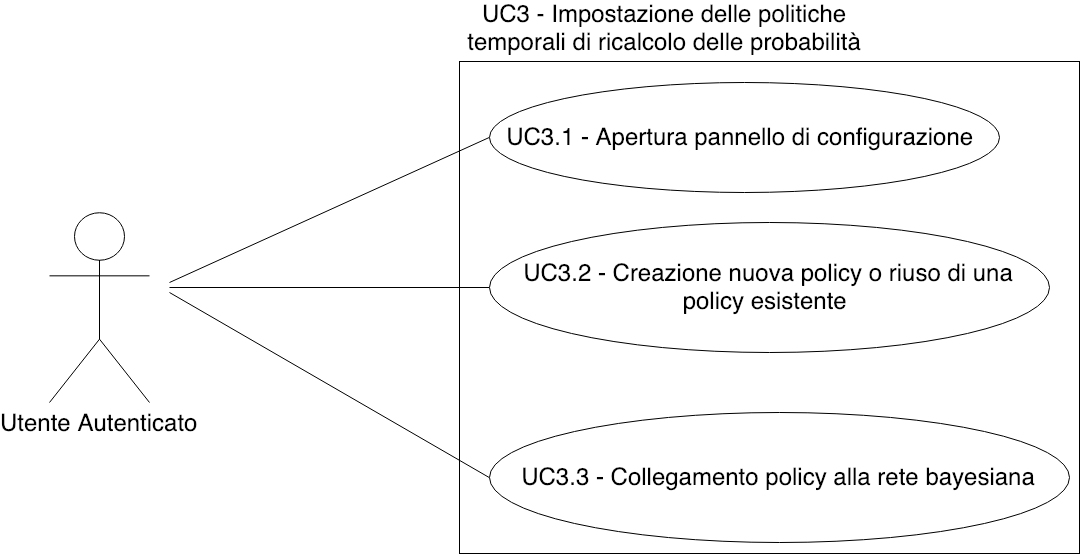
\includegraphics[scale=0.5]{./images/UC3.png}
\caption{UC3 - Selezione di una Politica Temporale di Ricalcolo delle Probabilità.}
\end{figure}

\begin{itemize}
	\item \textbf{Attore Primario}: Utente; 
	\item \textbf{Precondizione}: l'utente deve aver aggiunto il pannello "G\&B Panel";
	\item \textbf{Postcondizione}: l'utente ha collegato con successo la politica temporale da lui creata, per il ricalcolo delle probabilità della rete bayesiana, caricata in (\hyperref[UC1]{UC1 (§\ref*{UC1})});	
	\item \textbf{Scenario Principale:}
	\begin{enumerate}
		\item L'utente clicca il pulsante denominato "Politiche Temporali";
		\item L'utente crea una nuova politica temporale; 
		\item L'utente conferma la politica temporale realizzata.
	\end{enumerate}
	\item \textbf{Estensioni}: \hyperref[UC15]{UC15 (§\ref*{UC15})} estende \hyperref[UC3.3]{UC3.3 (§\ref*{UC3.3})}: l'utente visualizza un messaggio di errore nel caso in cui non abbia definito correttamente la politica temporale per il ricalcolo delle probabilità.
	
\end{itemize}

\subsubsection{UC3.1 - Click Pulsante "Politiche Temporali"}\label{UC3.1}
\begin{itemize}
	\item \textbf{Attore Primario}: Utente; 
	\item \textbf{Precondizione}: l'utente deve aver aggiunto il pannello "G\&B Panel";
	\item \textbf{Postcondizione}: l'utente accede al pannello di creazione della politica temporale;
	\item \textbf{Scenario Principale}: l'utente, tramite un click sul pulsante "Politiche Temporali", apre il pannello di configurazione. 
\end{itemize}

\subsubsection{UC3.2 - Creazione Nuova Politica Temporale}\label{UC3.2}

\begin{itemize}
	\item \textbf{Attore Primario}: Utente; 
	\item \textbf{Precondizione}: l'utente ha acceduto al pannello di creazione della politica temporale (\hyperref[UC3.1]{UC3.1 (§\ref*{UC3.1})});
	\item \textbf{Postcondizione}: l'utente ha realizzato la politica temporale per il ricalcolo delle probabilità desiderata;
	\item \textbf{Scenario Principale:}
	\begin{enumerate}
		\item L'utente visualizza due campi dati editabili che consentono la definizione di una politica temporale;
		\item L'utente inserisce, nel primo campo dati, il valore numerico del timeout ciclico per il ricalcolo delle probabilità condizionali associate ai nodi della rete bayesiana; 
		\item L'utente seleziona l'unità di misura temporale, attraverso una casella a scelta multipla che rappresenta il secondo campo dati editabile.
	\end{enumerate}
	
\end{itemize}

\subsubsection{UC3.3 - Conferma Politica Temporale}\label{UC3.3}
\begin{itemize}
	\item \textbf{Attore Primario}: Utente; 
	\item \textbf{Precondizione}: l'utente ha creato la politica temporale desiderata (\hyperref[UC3.2]{UC3.2 (§\ref*{UC3.2})});
	\item \textbf{Postcondizione}: l'utente ha confermato la politica temporale per il ricalcolo delle probabilità; 
	\item \textbf{Scenario Principale}: l'utente clicca il pusante "Conferma".
	\item \textbf{Estensioni}: \hyperref[UC15]{UC15 (§\ref*{UC15})}: l'utente visualizza un messaggio di errore nel caso in cui non abbia collegato alcun nodo ad un flusso dati.
\end{itemize}

\newpage

\subsection{UC4 - Visualizzazione Probabilità Associate ai Nodi non Collegati al Flusso}\label{UC4}

\begin{figure}[H]
\centering
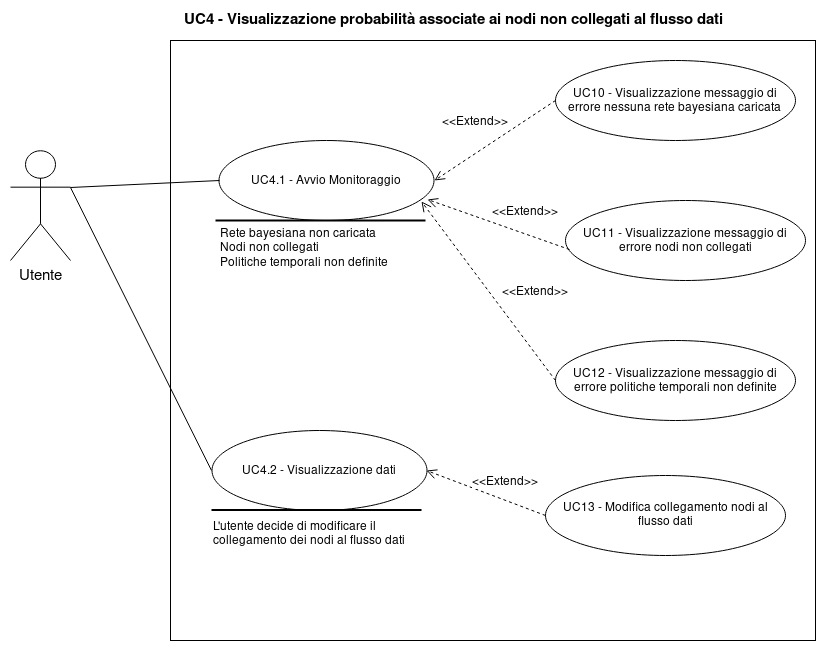
\includegraphics[scale=0.4]{./images/UC4.png}
\caption{UC4 - Visualizzazione delle Probabilità Associate ai Nodi non Collegati al Flusso}
\end{figure}

\begin{itemize}
\item \textbf{Attore Primario}: Utente;
\item \textbf{Precondizione}: l'utente deve aver effettuato il login nella piattaforma \textit{Grafana}, deve aver selezionato una dashboard e aggiunto il pannello "G\&B Panel";
%	\begin{enumerate}
%	\item L'utente ha collegato con successo alcuni nodi della rete bayesiana al flusso dati (\hyperref[UC2]{UC2 (§\ref*{UC2})});
%	\item L'utente ha definito le politiche temporali per il ricalcolo delle probabilità relative ai nodi della rete bayesiana (\hyperref[UC3]{UC3 (§\ref*{UC3})}).
%	\end{enumerate}
\item \textbf{Postcondizione:} il Sistema mantiene aggiornate, e visualizzabili da parte dell'utente, le misure di probabilità derivate dai nodi della rete bayesiana non collegati al flusso dati;
\item \textbf{Scenario Principale}: 
	\begin{enumerate}
	\item L'utente clicca il pulsante "Avvio Monitoraggio";
	\item L'utente visualizza i dati forniti dai nodi della rete bayesiana, tali dati sono una misura di probabilità 			associata ad ogni nodo della rete bayesiana non collegato al flusso dati (\hyperref[UC2]{UC2 (§\ref*{UC2})}). 				Tali probabilità vengono ricalcolate,mutando dinamicamente in base alle politiche temporali stabilite in 						\hyperref[UC3]{UC3 (§\ref*{UC3})}.
	\end{enumerate}
\item \textbf{Estensioni}:
	\begin{enumerate}
	\item \hyperref[UC10]{UC10 (§\ref*{UC10})} estende \hyperref[UC4.1]{UC4.1 (§\ref*{UC4.1})}: l'utente visualizza un messaggio di errore nel caso in cui non abbia caricato una rete bayesiana;
	\item \hyperref[UC11]{UC11 (§\ref*{UC11})} estende \hyperref[UC4.1]{UC4.1 (§\ref*{UC4.1})}: l'utente visualizza un messaggio di errore nel caso in cui non abbia collegato correttamente qualche nodo alla rete bayesiana;
	\item \hyperref[UC12]{UC12 (§\ref*{UC12})} estende \hyperref[UC4.1]{UC4.1 (§\ref*{UC4.1})}: l'utente visualizza un messaggio di errore nel caso in cui non abbia definito correttamente alcuna politica temporale per il ricalcolo delle probabilità;
	\item \hyperref[UC13]{UC13 (§\ref*{UC13})} estende \hyperref[UC4.2]{UC4.2 (§\ref*{UC4.2})}: la visualizzazione dei dati viene interrotta nel caso in cui l'utente decida di modificare il collegamento dei nodi della rete bayesiana al flusso dati.
	\end{enumerate}
\end{itemize}

\subsubsection{UC4.1 - Avvio Monitoraggio}\label{UC4.1}
\begin{itemize}
\item \textbf{Attore Primario:} utente;
\item \textbf{Precondizioni:}
	\begin{enumerate}
	\item L'utente ha collegato con successo alcuni nodi della rete bayesiana al flusso dati (\hyperref[UC2]{UC2 					(§\ref*{UC2})});
	\item L'utente ha definito le politiche temporali per il ricalcolo delle probabilità relative ai nodi della rete bayesiana (\hyperref[UC3]{UC3 (§\ref*{UC3})}).
	\end{enumerate}
\item \textbf{Postcondizione:} il pannello espone all'utente la lista di nodi della rete bayesiana caricata ed i corrispondenti dati ad essi associati;
\item \textbf{Scenario Principale:}
	\begin{enumerate}
	\item L'utente clicca il pulsante denominato "Avvio Monitoraggio";
	\item Il pulsante "Avvio Monitoraggio" scompare, venendo sostituito dalla lista lista di nodi della rete 	bayesiana associati ai corrispondenti dati di monitoraggio.
	\end{enumerate}
\item \textbf{Estensioni:}
	\begin{enumerate}
	\item \hyperref[UC11]{UC11 (§\ref*{UC11})}: l'utente visualizza un messaggio di errore nel caso in cui non abbia caricato alcuna rete bayesiana (\hyperref[UC1]{UC1 (§\ref*{UC1})});
	\item \hyperref[UC12]{UC12 (§\ref*{UC12})}: l'utente visualizza un messaggio di errore nel caso in cui non abbia collegato correttamente qualche nodo alla rete bayesiana (\hyperref[UC2]{UC2 (§\ref*{UC2})});
	\item \hyperref[UC13]{UC13 (§\ref*{UC13})}: l'utente visualizza un messaggio di errore nel caso in cui non abbia definito correttamente alcuna politica temporale per il ricalcolo delle probabilità (\hyperref[UC3]{UC3 (§\ref*{UC3})}).
	\end{enumerate}
\end{itemize}

\subsubsection{UC4.2 - Visualizzazione Dati}\label{UC4.2}
\begin{itemize}
\item \textbf{Attore Primario:} utente;
\item \textbf{Precondizione:} l'utente ha avviato correttamente il monitoraggio del flusso dati.
\item \textbf{Postcondizione:} il Sistema mantiene aggiornate, e visualizzabili da parte dell'utente, le misure di probabilità derivate dai nodi della rete bayesiana non collegati al flusso dati;
\item \textbf{Scenario Principale:} l'utente visualizza l'andamento delle probabilità dinamiche associate ai nodi 			della rete bayesiana non collegati direttamente al flusso dati. Il sistema aggiorna costantemente i dati forniti dalla rete bayesiana, effettuando l'operazione di ricalcolo delle probabilità associate ai nodi della rete non collegati al flusso dati. Tale operazione di ricalcolo delle probabilità viene eseguita allo scadere del timeout ciclico rappresentato dalla politica temporale stabilita in \hyperref[UC3]{UC3 (§\ref*{UC3})}, oppure, nel caso siano state definite in sede di collegamento nodi (\hyperref[UC2.2.4]{UC2.2.4 (§\ref*{UC2.2.4})}), ogni volta che una soglia critica viene attivata dai dati monitorati;
\item \textbf{Estensioni:} \hyperref[UC13]{UC13 (§\ref*{UC13})}: la visualizzazione dei dati viene interrotta nel 			caso in cui l'utente decida di modificare il collegamento dei nodi della rete bayesiana al flusso dati.
\end{itemize}

\newpage

\subsection{UC5 - Definizione di un Alert sui Nodi non Collegati il Flussi Dati}\label{UC5}

\begin{figure}[H]
	\centering
	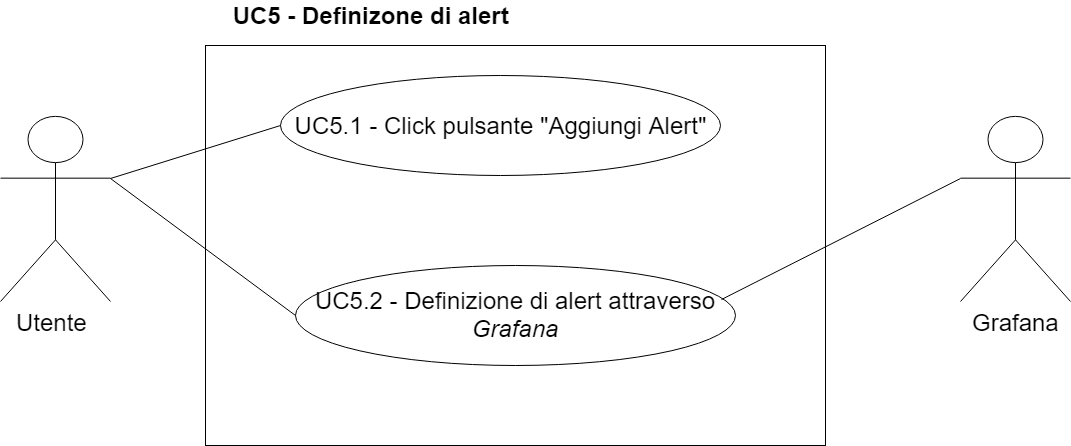
\includegraphics[scale=0.3]{./images/UC5.png}
	\caption{UC5 - Definizione di un Alert sui Nodi non Collegati al Flusso dei Dati}
\end{figure}

\begin{itemize}
	\item \textbf{Attore Primario}: Utente;
	\item \textbf{Precondizione}:
	l'utente ha avviato con successo il monitoraggio del flusso dati (\hyperref[UC4]				{UC4 (§\ref*{UC4})}) e visualizza correttamente le probabilità associate ai nodi della rete bayesiana;
	\item \textbf{Postcondizione}: l'utente ha aggiunto un alert per i nodi non collegati al flusso di dati;
	\item \textbf{Scenario Principale}:
	\begin{enumerate}
		\item \hyperref[UC5.1]{UC5.1 (§\ref*{UC5.1})}  L'utente clicca sul pulsante "Aggiungi Alert";
		\item \hyperref[UC5.2]{UC5.2 (§\ref*{UC5.2})} L'utente, attraverso le impostazioni messe a disposizione della piattaforma \textit{Grafana}, definisce l'alert desiderato.
	\end{enumerate}
	
\end{itemize}

\subsubsection{UC5.1 - Click Pulsante "Aggiungi Alert"}\label{UC5.1}
\begin{itemize}
	\item \textbf{Attore Primario}: Utente;
	\item \textbf{Precondizione}: l'utente deve aver aggiunto il pannello "G\&B Panel";
	\item \textbf{Postcondizione}: l'utente viene condotto alle impostazioni di edit del pannello 
	"G\&B Panel", sotto la voce Alert;
	\item \textbf{Scenario Principale}: l'utente clicca il bottone "Aggiungi Alert".
\end{itemize}

\subsubsection{UC5.2 - Definizione di Alert Attraverso \textit{Grafana}}\label{UC5.2}
\begin{itemize}
	\item \textbf{Attore Primario}: Utente;
	\item \textbf{Attore secondario}: \textit{Grafana};
	\item \textbf{Precondizione}: l'utente ha cliccato il pulsante "Aggiungi alert" \hyperref[UC5.1]{UC5.1 (§\ref*{UC5.1})};
	\item \textbf{Postcondizione}: l'utente ha creato l'alert attraverso le impostazioni di \textit{Grafana};
	\item \textbf{Scenario Principale}: l'utente, attraverso le impostazioni messe a disposizione da \textit{Grafana}, definisce l'alert desiderato.
\end{itemize}

\newpage

\subsection{UC6 - Rimozione Alert}\label{UC6}

\begin{figure}[H]
	\centering
	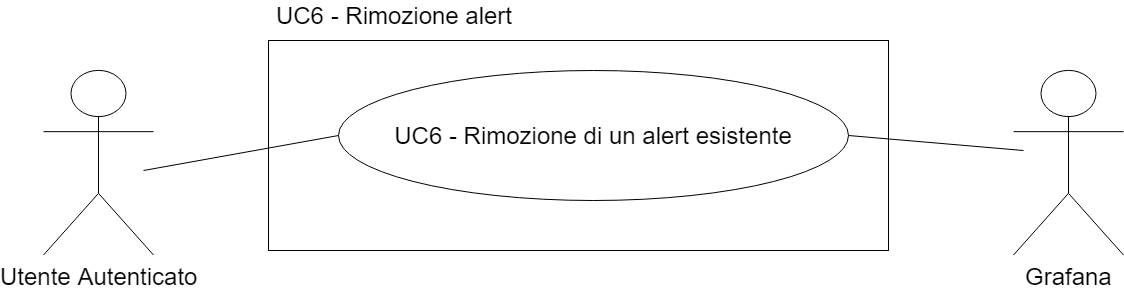
\includegraphics[scale=0.4]{./images/UC6.png}
	\caption{UC6 - Rimozione Alert}
\end{figure}

\begin{itemize}
	\item \textbf{Attore Primario}: Utente;
	\item \textbf{Precondizione:} l'utente visualizza il pannello degli alert \hyperref[UC7]{UC7 (§\ref*{UC7})};
	\item \textbf{Postcondizione}: l'utente ha rimosso l'alert associato al nodo non collegato al flusso dati;
	\item \textbf{Scenario Principale}: 
	\begin{enumerate}
		\item \hyperref[UC6.1]{UC6.1 (§\ref*{UC6.1})} L'utente clicca sull'alert che desidera eliminare;
		\item \hyperref[UC6.2]{UC6.2 (§\ref*{UC6.2})} L'utente, attraverso le impostazioni di \textit{Grafana}, elimina l'alert.
	\end{enumerate}
\end{itemize}

\subsubsection{UC6.1 - Selezione Alert da Eliminare}\label{UC6.1}
\begin{itemize}
	\item \textbf{Attore Primario}: Utente;
	\item \textbf{Precondizione}:  l'utente visualizza il pannello degli alert \hyperref[UC7]{UC7 (§\ref*{UC7})};
	\item \textbf{Postcondizione}: l'utente viene condotto nella sezione di edit del pannello "G\&B Panel", sotto la voce Alert;
	\item \textbf{Scenario Principale}: l'utente clicca sul nominativo dell'alert che desidera rimuovere.
\end{itemize}

\subsubsection{UC6.2 - Rimozione di Alert Attraverso \textit{Grafana}}\label{UC6.2}
\begin{itemize}
	\item \textbf{Attore Primario}: Utente;
	\item \textbf{Attore secondario}: \textit{Grafana};
	\item \textbf{Precondizione}:  l'utente ha selezionato l'alert che vuole eliminare \hyperref[UC6.1]{UC6.1 (§\ref*{UC6.1})};
	\item \textbf{Postcondizione}: l'alert desiderato è stato eliminato;
	\item \textbf{Scenario Principale}: l'utente elimina l'alert attraverso le impostazione messe a disposizione da \textit{Grafana}.
\end{itemize}

\pagebreak

\subsection{UC7 - Visualizzazione Alert}\label{UC7}

\begin{figure}[H]
	\centering
	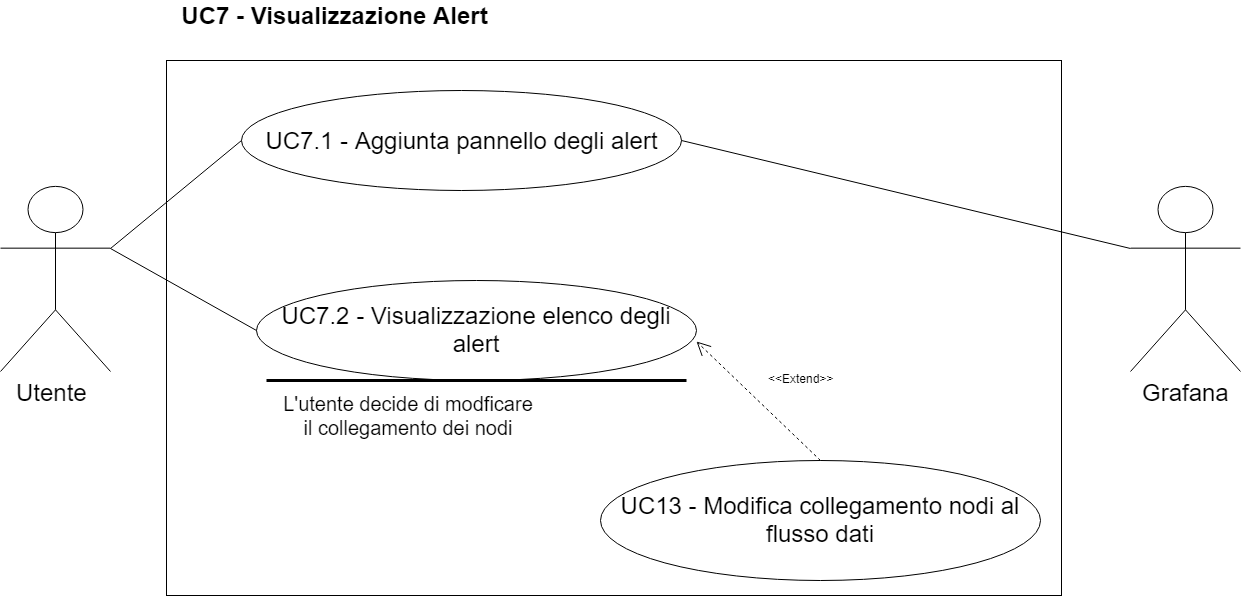
\includegraphics[scale=0.5]{./images/UC7.png}
	\caption{UC7 - Visualizzazione di un Alert}
\end{figure}

\begin{itemize}
	\item \textbf{Attore Primario}: Utente;
	\item \textbf{Attore secondario}: \textit{Grafana};
	\item \textbf{Precondizioni}: l'utente ha definito correttamente almeno un alert (\hyperref[UC5]{UC5(§\ref*{UC5})});
	\item \textbf{Postcondizioni}: l'utente visualizza l'elenco degli alert definiti e il relativo stato;
	\item \textbf{Scenario Principale}:
	\begin{enumerate}
		\item (\hyperref[UC7.1]{UC7.1(§\ref*{UC7.1})}) L'utente attraverso le impostazioni messe a disposizione di \textit{Grafana}, aggiunge il pannello di visualizzazione degli alert.
		\item (\hyperref[UC7.2]{UC7.2(§\ref*{UC7.2})}) L'utente visualizza lo stato degli alert definiti sui nodi non collegati al flusso di dati.
	\end{enumerate}
	\item \textbf{Estensioni:} \hyperref[UC13]{UC13 (§\ref*{UC13})} estende \hyperref[UC7.2]{UC7.2 (§\ref*{UC7.2})}: la visualizzazione degli alert viene interrotta nel caso in cui l'utente decida di modificare il collegamento dei nodi della rete bayesiana al flusso dati.
\end{itemize}

\newpage

\subsubsection{UC7.1 - Aggiunta Pannello degli Alert }\label{UC7.1}
\begin{itemize}
	\item \textbf{Attore Primario}: Utente;
	\item \textbf{Attore secondario}: \textit{Grafana};
	\item \textbf{Precondizione}: l'utente ha aggiunto il pannello "G\&B Panel";
	\item \textbf{Postcondizione}: l'utente ha aggiunto il pannello di visualizzazione degli alert;
	\item \textbf{Scenario Principale}: l'utente, attraverso le impostazioni messe a disposizione di \textit{Grafana}, aggiunge il pannello di visualizzazione degli alert;
\end{itemize}

\subsubsection{UC7.2 - Visualizzazione Elenco degli Alert}\label{UC7.2}
\begin{itemize}
	\item \textbf{Attore Primario}: Utente;
	\item \textbf{Precondizione}:  l'utente ha aggiunto il pannello degli alert \hyperref[UC7.1]{UC7.1 (§\ref*{UC7.1})}.
	\item \textbf{Postcondizione}: l'utente visualizza l'elenco degli alert definiti in  \hyperref[UC5]{UC5 (§\ref*{UC5})}.
	\item \textbf{Scenario Principale}: l'utente visualizza l'elenco degli alert definiti sui nodi non collegati al flusso di dati e il relativo stato;
	\item \textbf{Estensioni:} \hyperref[UC13]{UC13 (§\ref*{UC13})} la visualizzazione degli alert viene interrotta nel caso in cui l'utente decida di modificare il collegamento dei nodi della rete bayesiana al flusso dati.
\end{itemize}


\pagebreak

\subsection{UC8 - Visualizzazione Messaggio d'Errore Selezione Rete Bayesiana}\label{UC8}
\begin{itemize}
\item \textbf{Attore Primario}: Utente;
\item \textbf{Precondizione}: l'utente ha selezionato una rete da aggiungere ed ha cliccato il pulsante "Aggiungi", per confermare la rete. La rete selezionata dall'utente è errata per formato o per struttura;
\item \textbf{Postcondizione}: l'utente visualizza l'errore, viene quindi riportato alla finestra di selezione del file della rete bayesiana (\hyperref[UC1.2]{UC1.2 (§\ref*{UC1.2})});
\item \textbf{Scenario Principale:} 
	\begin{enumerate}
	\item L'utente visualizza un messaggio di errore in cui è segnalato il fatto che la struttura del file di definizione della rete bayesiana, caricato in (\hyperref[UC1.2]{UC1.2 (§\ref*{UC1.2})}, non è corretta;
	\item L'utente clicca il pulsante con etichetta "OK".
	\end{enumerate}
\end{itemize}

\pagebreak

\subsection{UC9 - Visualizzazione Messaggio di Errore Nessun Nodo Collegato}\label{UC9}
\begin{itemize}
\item \textbf{Attore Primario}: Utente;
\item \textbf{Precondizione}: l'utente ha confermato il collegamento dei nodi al flusso dati (\hyperref[UC2.2]{UC2.2 (§\ref*{UC2.2})}), senza averne effettivamente collegato alcuno;
\item \textbf{Postcondizione}: l'utente visualizza l'errore;
\item \textbf{Scenario Principale}: 
	\begin{enumerate}
	\item L'utente visualizza un messaggio di errore in cui è segnalato il fatto che non sia stato collegato alcun 				nodo al flusso dati durante \hyperref[UC2]{UC2 (§\ref*{UC2})};
	\item L'utente clicca il pulsante con etichetta "OK".
	\end{enumerate}
\end{itemize}

\pagebreak

\subsection{UC10 - Visualizzazione Messaggio di Errore Nessuna Rete Bayesiana Caricata}\label{UC10}
\begin{itemize}
\item \textbf{Attore Primario}: Utente;
\item \textbf{Precondizione}: l'utente ha avviato il monitoraggio del flusso dati (\hyperref[UC4.1]{UC4.1 (§\ref*{UC4.1})}), senza aver preventivamente caricato alcuna rete bayesiana (\hyperref[UC1]{UC1 (§\ref*{UC1})}).
\item \textbf{Postcondizione}: l'utente visualizza l'errore;
\item \textbf{Scenario Principale}: 
	\begin{enumerate}
	\item L'utente visualizza un messaggio di errore in cui è segnalato il fatto che non sia stata preventivamente 				caricata alcuna rete bayesiana;
	\item L'utente clicca il pulsante con etichetta "OK".
	\end{enumerate}
\end{itemize}

\pagebreak

\subsection{UC11 - Visualizzazione Messaggio di Errore Nodi non Collegati}\label{UC11}
\begin{itemize}
\item \textbf{Attore Primario}: Utente;
\item \textbf{Precondizione}: l'utente ha avviato il monitoraggio del flusso dati (\hyperref[UC4.1]{UC4.1 							(§\ref*{UC4.1})}), senza aver preventivamente collegato alcuni nodi della rete bayesiana al flusso dati 							(\hyperref[UC2]{UC2 (§\ref*{UC2})}).
\item \textbf{Postcondizione}: l'utente visualizza l'errore;
\item \textbf{Scenario Principale}: 
	\begin{enumerate}
	\item L'utente visualizza un messaggio di errore in cui è segnalato il fatto che non siano stati collegati 						correttamente dei nodi della rete bayesiana al flusso dati;
	\item L'utente clicca il pulsante con etichetta "OK".
	\end{enumerate}
\end{itemize}

\pagebreak

\subsection{UC12 - Visualizzazione Messaggio di Errore Politiche Temporali non Definite}\label{UC12}
\begin{itemize}
\item \textbf{Attore Primario}: Utente;
\item \textbf{Precondizione}: l'utente ha avviato il monitoraggio del flusso dati (\hyperref[UC4.1]{UC4.1 							(§\ref*{UC4.1})}), senza aver preventivamente definito correttamente alcuna politica temporale per il ricalcolo delle probabilità (\hyperref[UC3]{UC3 (§\ref*{UC3})}).
\item \textbf{Postcondizione}: l'utente visualizza l'errore;
\item \textbf{Scenario Principale}: 
	\begin{enumerate}
	\item L'utente visualizza un messaggio di errore in cui è segnalato il fatto che non sia stata definita alcuna 				politica temporale per il ricalcolo delle probabilità;
	\item L'utente clicca il pulsante con etichetta "OK".
	\end{enumerate}
\end{itemize}

\pagebreak

\subsection{UC13 - Modifica Collegamento Nodi al Flusso Dati}\label{UC13}

\begin{figure}[H]
\centering
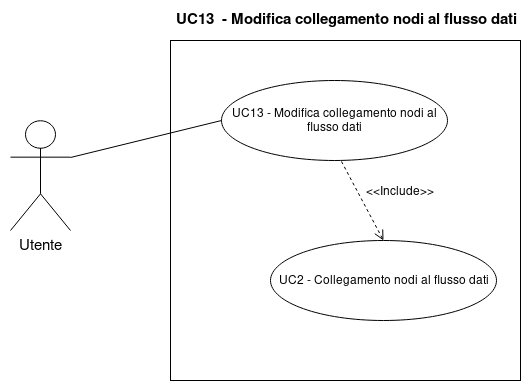
\includegraphics[scale=0.6]{./images/UC13.png}
\caption{UC12 - Modifica Collegamento Nodi al Flusso Dati}
\end{figure}


\begin{itemize}
\item \textbf{Attore Primario:} utente;
\item \textbf{Precondizione:} l'utente ha collegato con successo alcuni nodi della rete bayesiana al flusso dati (\hyperref[UC2]{UC2 (§\ref*{UC2})});
\item \textbf{Postcondizioni:} 
	\begin{enumerate}
	\item L'utente ha modificato con successo i nodi della rete bayesiana collegati al flusso dati;
	\item La visualizzazione dei dati forniti dai nodi della rete bayesiana (\hyperref[UC4]{UC4 (§\ref*{UC4})}) viene interrotta, se avviata. Di conseguenza torna visibile il pulsante "Avvio Monitoraggio";
	\item Gli alert definiti in \hyperref[UC5]{UC5 (§\ref*{UC5})} vengono eliminati, se presenti.
	\end{enumerate}
\item \textbf{Scenario Principale:}
	\begin{enumerate}
	\item (\hyperref[UC13.1]{UC13.1 (§\ref*{UC13.1})}) l'utente clicca il pulsante "Modifica Collegamento Nodi";
	\item (\hyperref[UC2]{UC2 (§\ref*{UC2})}) l'utente effettua nuovamente il collegamento dei nodi.
	\end{enumerate}
\end{itemize}

\subsubsection{UC13.1 - Click Pulsante "Modifica Collegamento Nodi"}\label{UC13.1}
\begin{itemize}
\item \textbf{Attore Primario:} utente;
\item \textbf{Precondizione:} l'utente ha collegato con successo alcuni nodi della rete bayesiana al flusso dati 			(\hyperref[UC2]{UC2 (§\ref*{UC2})});
\item \textbf{Postcondizione:} il pannello contenente la lista dei nodi torna ad essere interagibile da parte dell'utente.
\item \textbf{Scenario Principale:} l'utente clicca il pulsante denominato: "Modifica Collegamento Nodi".
\end{itemize}
\newpage

\subsection{UC14 - Visualizzazione Messaggio di Errore Nessuna Soglia Impostata}\label{UC14}
\begin{itemize}
\item \textbf{Attore Primario}: Utente;
\item \textbf{Precondizione}: l'utente ha confermato le scelte per il collegamento di un dato nodo ad un flusso 				dati (\hyperref[UC2.2.4]{UC2.2.4 (§\ref*{UC2.2.4})}), senza aver impostato correttamente una soglia per lo stesso 	(\hyperref[UC2.2.3]{UC2.2.3 (§\ref*{UC2.2.3})});
\item \textbf{Postcondizioni}: 
	\begin{enumerate}
	\item L'utente visualizza l'errore;
	\item Le scelte dell'utente non vengono confermate.
	\end{enumerate}
\item \textbf{Scenario Principale}: 
	\begin{enumerate}
	\item L'utente visualizza un messaggio di errore in cui sono indicati gli errori commessi;
	\item L'utente clicca il pulsante con etichetta "OK".
	\end{enumerate}
\end{itemize}

\pagebreak

\subsection{UC15 - Visualizzazione Messaggio di Errore Politica Temporale non Configurata Correttamente}\label{UC15}
\begin{itemize}
\item \textbf{Attore Primario}: Utente;
\item \textbf{Precondizione}: l'utente ha confermato le scelte per la selezione di una politica temporale per il ricalcolo delle probabilità (\hyperref[UC3.3]{UC3.3 (§\ref*{UC3.3})}), senza averla definita correttamente (\hyperref[UC3.2]{UC3.2 (§\ref*{UC3.2})});
\item \textbf{Postcondizioni}: 
	\begin{enumerate}
	\item L'utente visualizza l'errore;
	\item La politica temporale non viene impostata.
	\end{enumerate}
\item \textbf{Scenario Principale}: 
	\begin{enumerate}
	\item L'utente visualizza un messaggio di errore in cui sono indicati gli errori commessi;
	\item L'utente clicca il pulsante con etichetta "OK".
	\end{enumerate}
\end{itemize}



